\label{Evaluation}

In order to evaluate the performance of both algorithms, we implemented them in C++ \footnote{\url{https://github.com/jsilll/crc}} using the Boost Graph Library's (BGL) \footnote{\url{https://www.boost.org/doc/libs/1_82_0/libs/graph/doc/index.html}} graph data structure. This allowed us to easily generate random graph instances and to use the BGL's built-in functions to visualize the graphs and the k-cores. Moreover, having both algorithms implemented in the same language and using the same graph data structure allowed us to compare them in a fair way.

To benchmark the algorithms, we used various graphs from the Stanford Network Analysis Project (SNAP) \footnote{\url{https://snap.stanford.edu/data/}}. We ran the algorithms for all the $k$ values between 1 and the maximum k-core of the graph. The results are presented in figures \ref{fig:Amazon_CitPatents} and \ref{fig:skitter_google_wiki}.

All the benchmarks were run on a computer with an Intel Core i5-8250U CPU and 8GB of RAM. The operating system was Fedora 38. The compiler used was Clang 16.0.4 with the \texttt{-O3} and \texttt{-march=native} compile flags.
\begin{figure}[H]
    \centering
    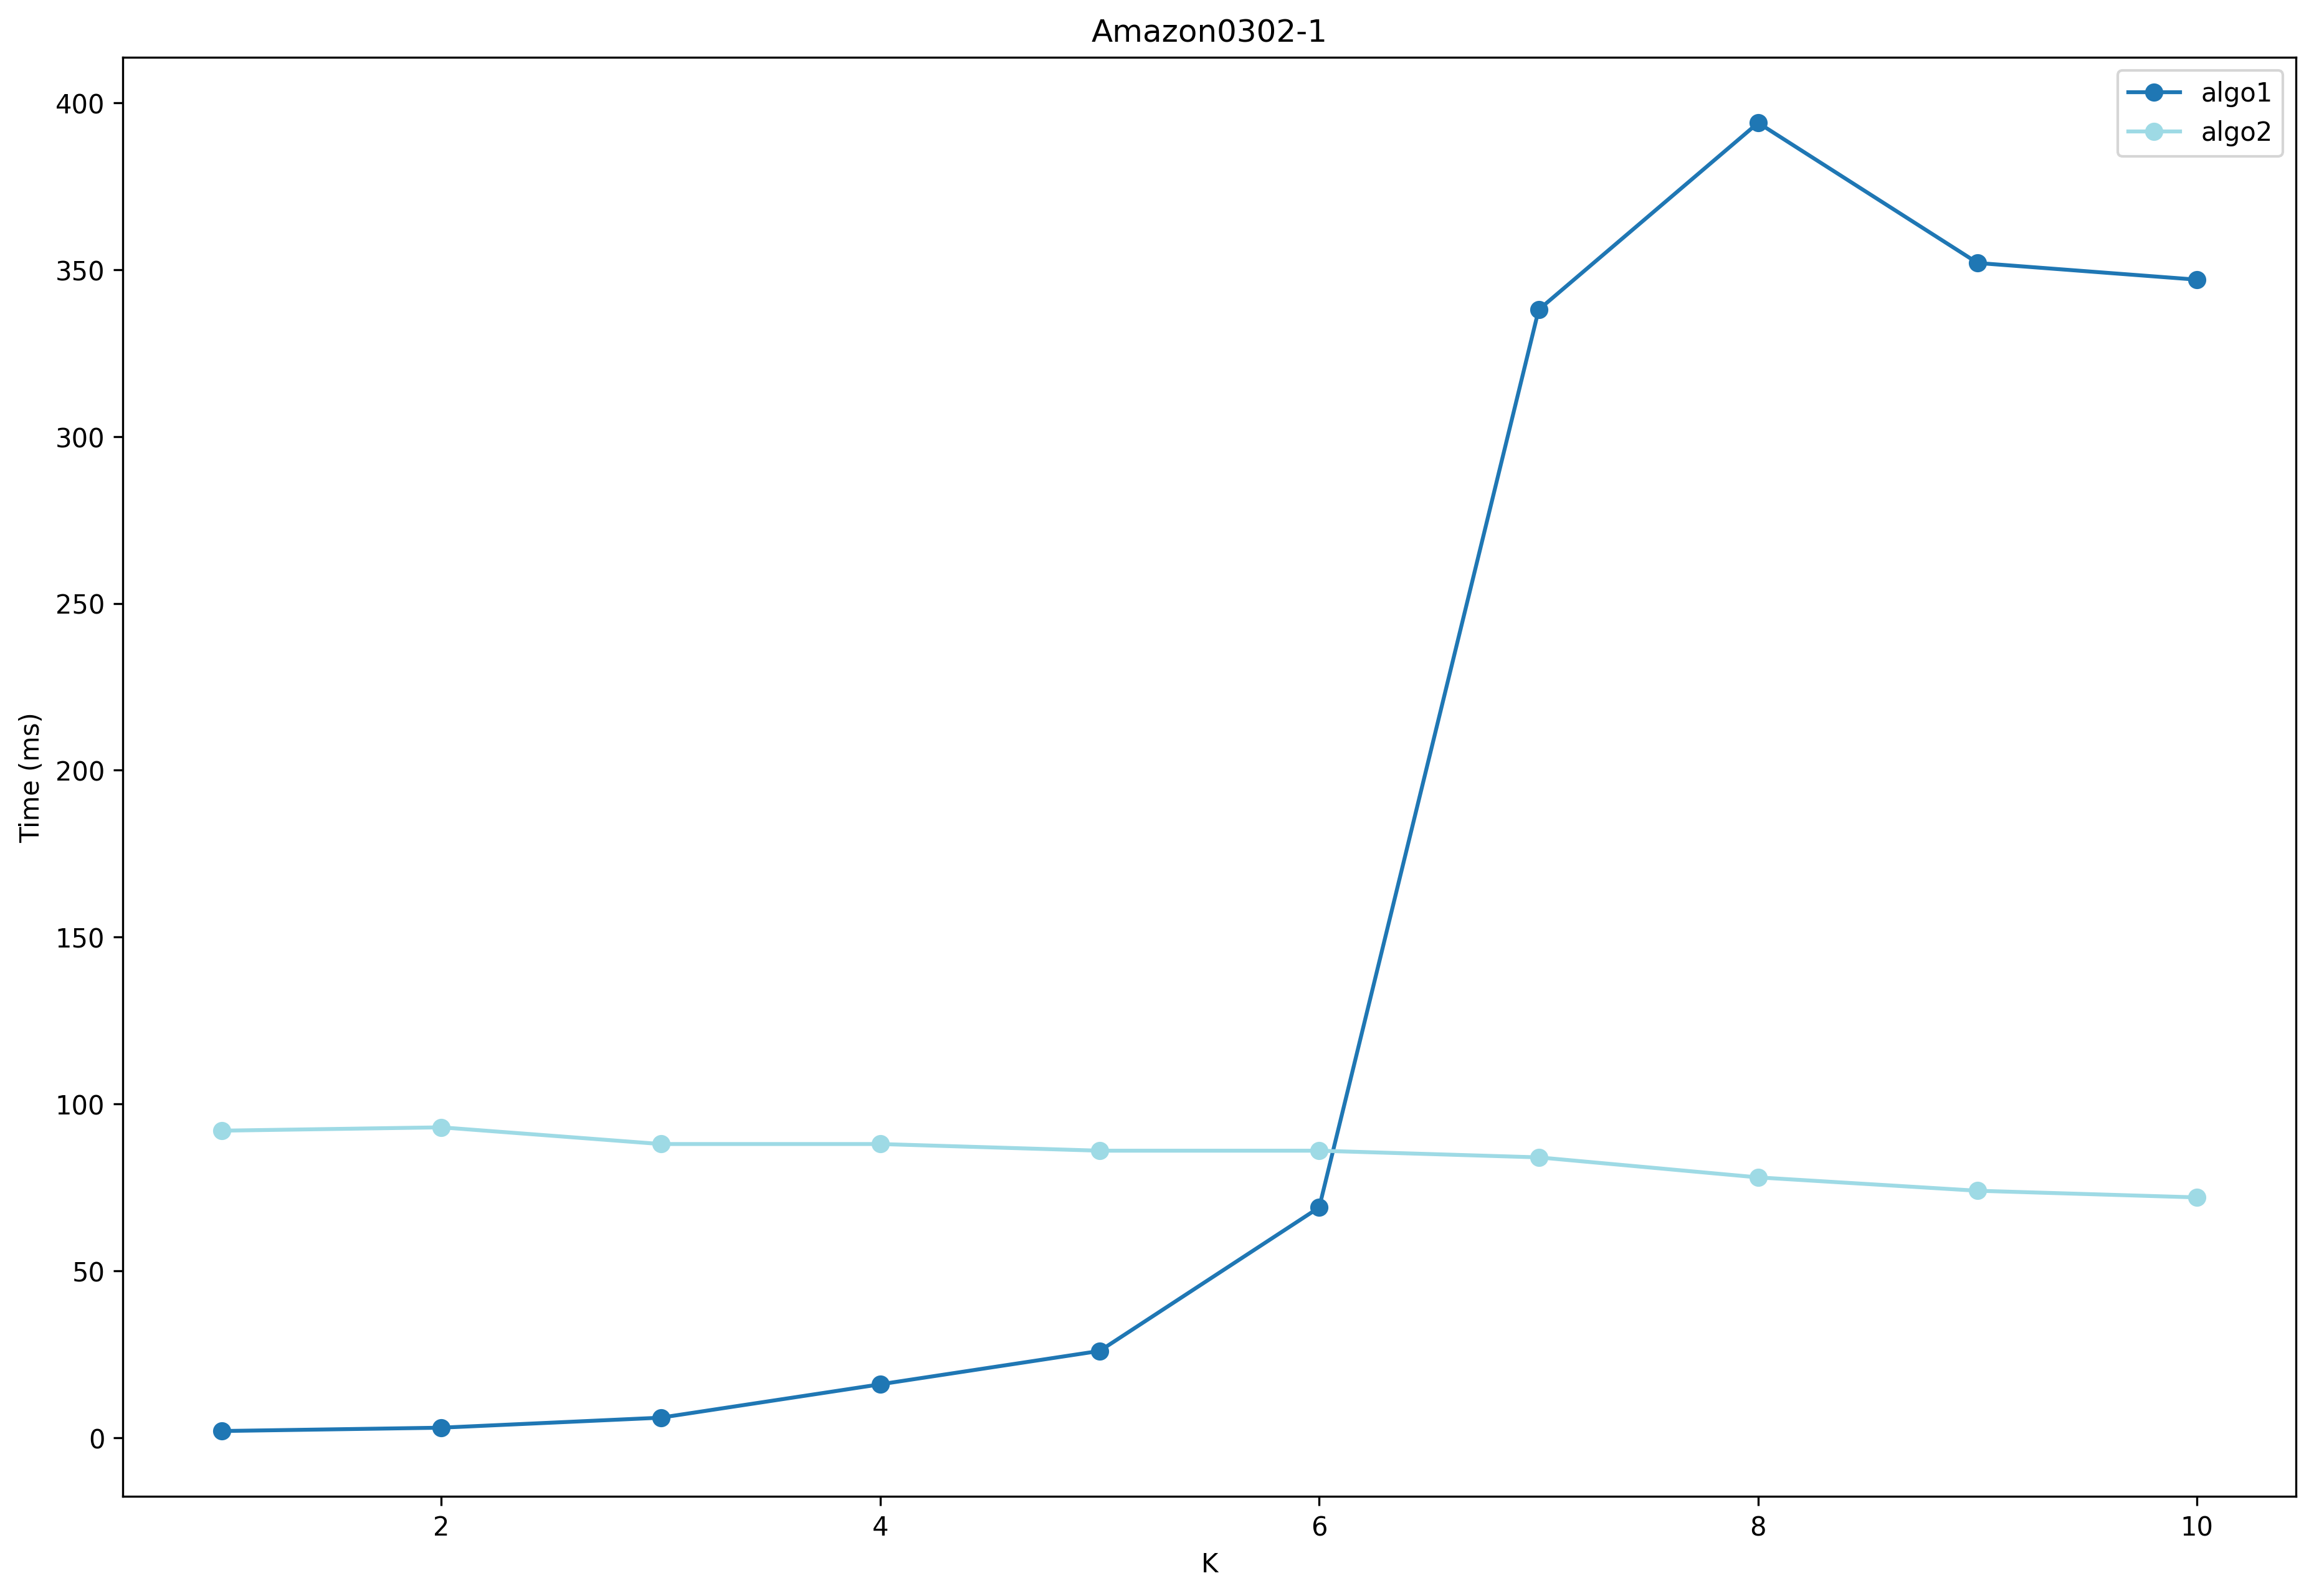
\includegraphics[width=0.48\textwidth]{Figures/Amazon0302-1.png}
    \includegraphics[width=0.48\textwidth]{Figures/cit-Patents.png}
    \caption{Amazon and cit-Patents benchmarks}
    \label{fig:Amazon_CitPatents}
\end{figure}

\begin{figure}[H]
	\centering
	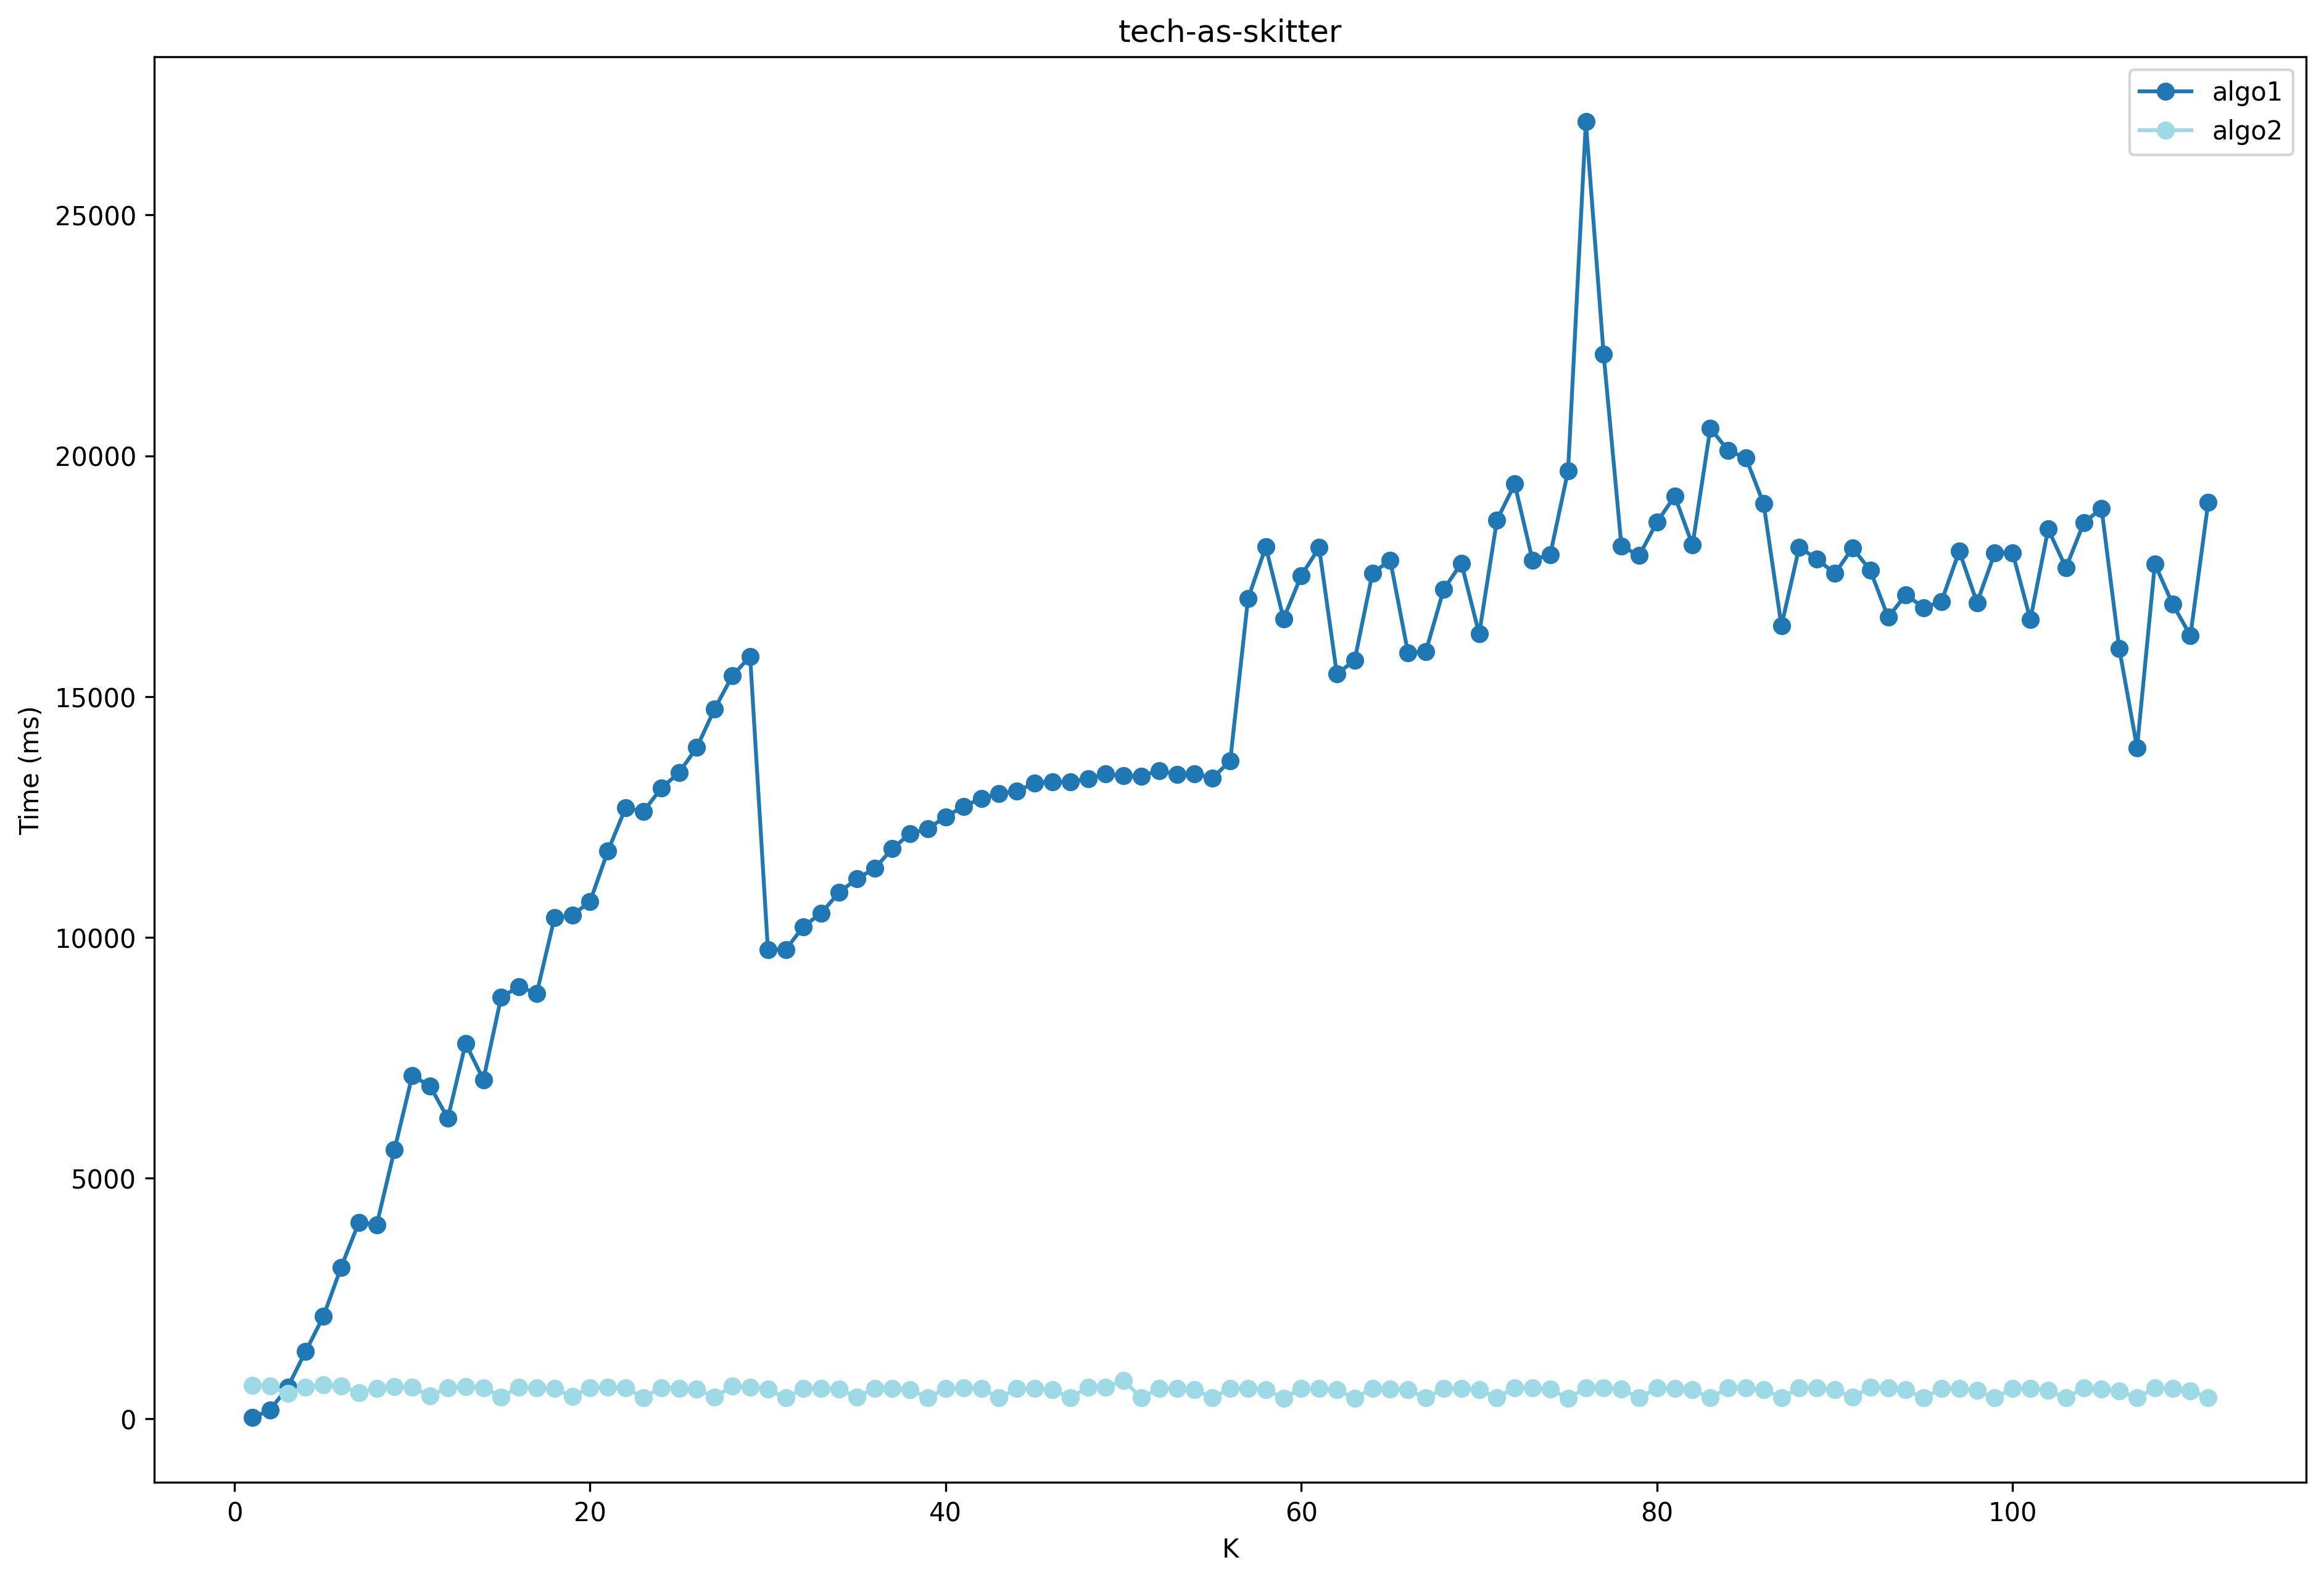
\includegraphics[width=0.48\textwidth]{Figures/tech-as-skitter.png} 
        \includegraphics[width=0.48\textwidth]{Figures/web-Google.png} 
        \includegraphics[width=0.48\textwidth]{Figures/WikiTalk.png} 
        \caption{tech-as-skitter, web-Google and WikiTalk benchmarks}
        \label{fig:skitter_google_wiki}
\end{figure}

The results consistently demonstrate that the depth-first search-based algorithm outperforms the degree-pruning algorithm significantly. Several factors contribute to this performance difference. 

To begin with, the process of removing vertices and edges in the degree-pruning algorithm is computationally expensive. In contrast, the depth-first search-based algorithm simply maintains information about vertex degrees and visited vertices, which is a considerably simpler task that exploits locality.

Secondly, the degree-pruning algorithm allows a node to be inserted multiple times, leading to a larger queue that needs to be processed. In contrast, the DFS based algorithm traverses each node only once by effectively tracking visited nodes.

Lastly, the degree-pruning algorithm is akin to a breadth-first search approach tailored to uncover the k-cores of a graph. Given this resemblance and the specific benchmarks considered, opting for a depth-first search-based algorithm offers performance benefits, resulting in consistently faster execution times than the degree-pruning algorithm.